
\section{Software}
O Blender\footnote{www.blender.org} é um pacote de software de computação gráfica 3D, gratuito e de código aberto, usado, por exemplo, na criação de animações, efeitos visuais, modelos tridimensionais impressos, aplicações 3D interativas e jogos digitais. Neste contexto, o software suporta modelagem 3D, texturização, animação, simulação de fluidos e fumaça, simulação de partículas, renderização, entre outras funcionalidades. \\

O software é mantido pela Blender Foundation, uma instituição sem fins lucrativos, cuja principal fonte de renda é a criação de material de treinamento e o oferecimento de cursos e treinamentos presenciais em Amsterdã. O pacote tem uma grande base instalada, mas é difícil estimar o número de usuários ativos - o número de {\it downloads} a partir do {\it site} oficial é superior a 3 milhões por ano. A distribuição oficial, disponibilizada sob a licença GNU-GPL\footnote{http://www.gnu.org/licenses/gpl.html}, contempla as plataformas Linux, Mac OS X e Windows, para plataformas de 32 e 64 bits. \\

A interface padrão do usuário prioriza a produção de animações 3D, porém é altamente configurável, e permite um ajuste fino de acordo com as necessidades de cada usuário, embora a curva de aprendizagem possa ser substancial. Uma interface programável (API) é oferecida para {\it scripts} escritos em Python, permitindo a automação de várias tarefas dentro do software. Na Figura \ref{blender_gui}, a interface do programa é mostrada. \\ 

%figura aqui!! :-P
\begin{figure}[!htb]
\center
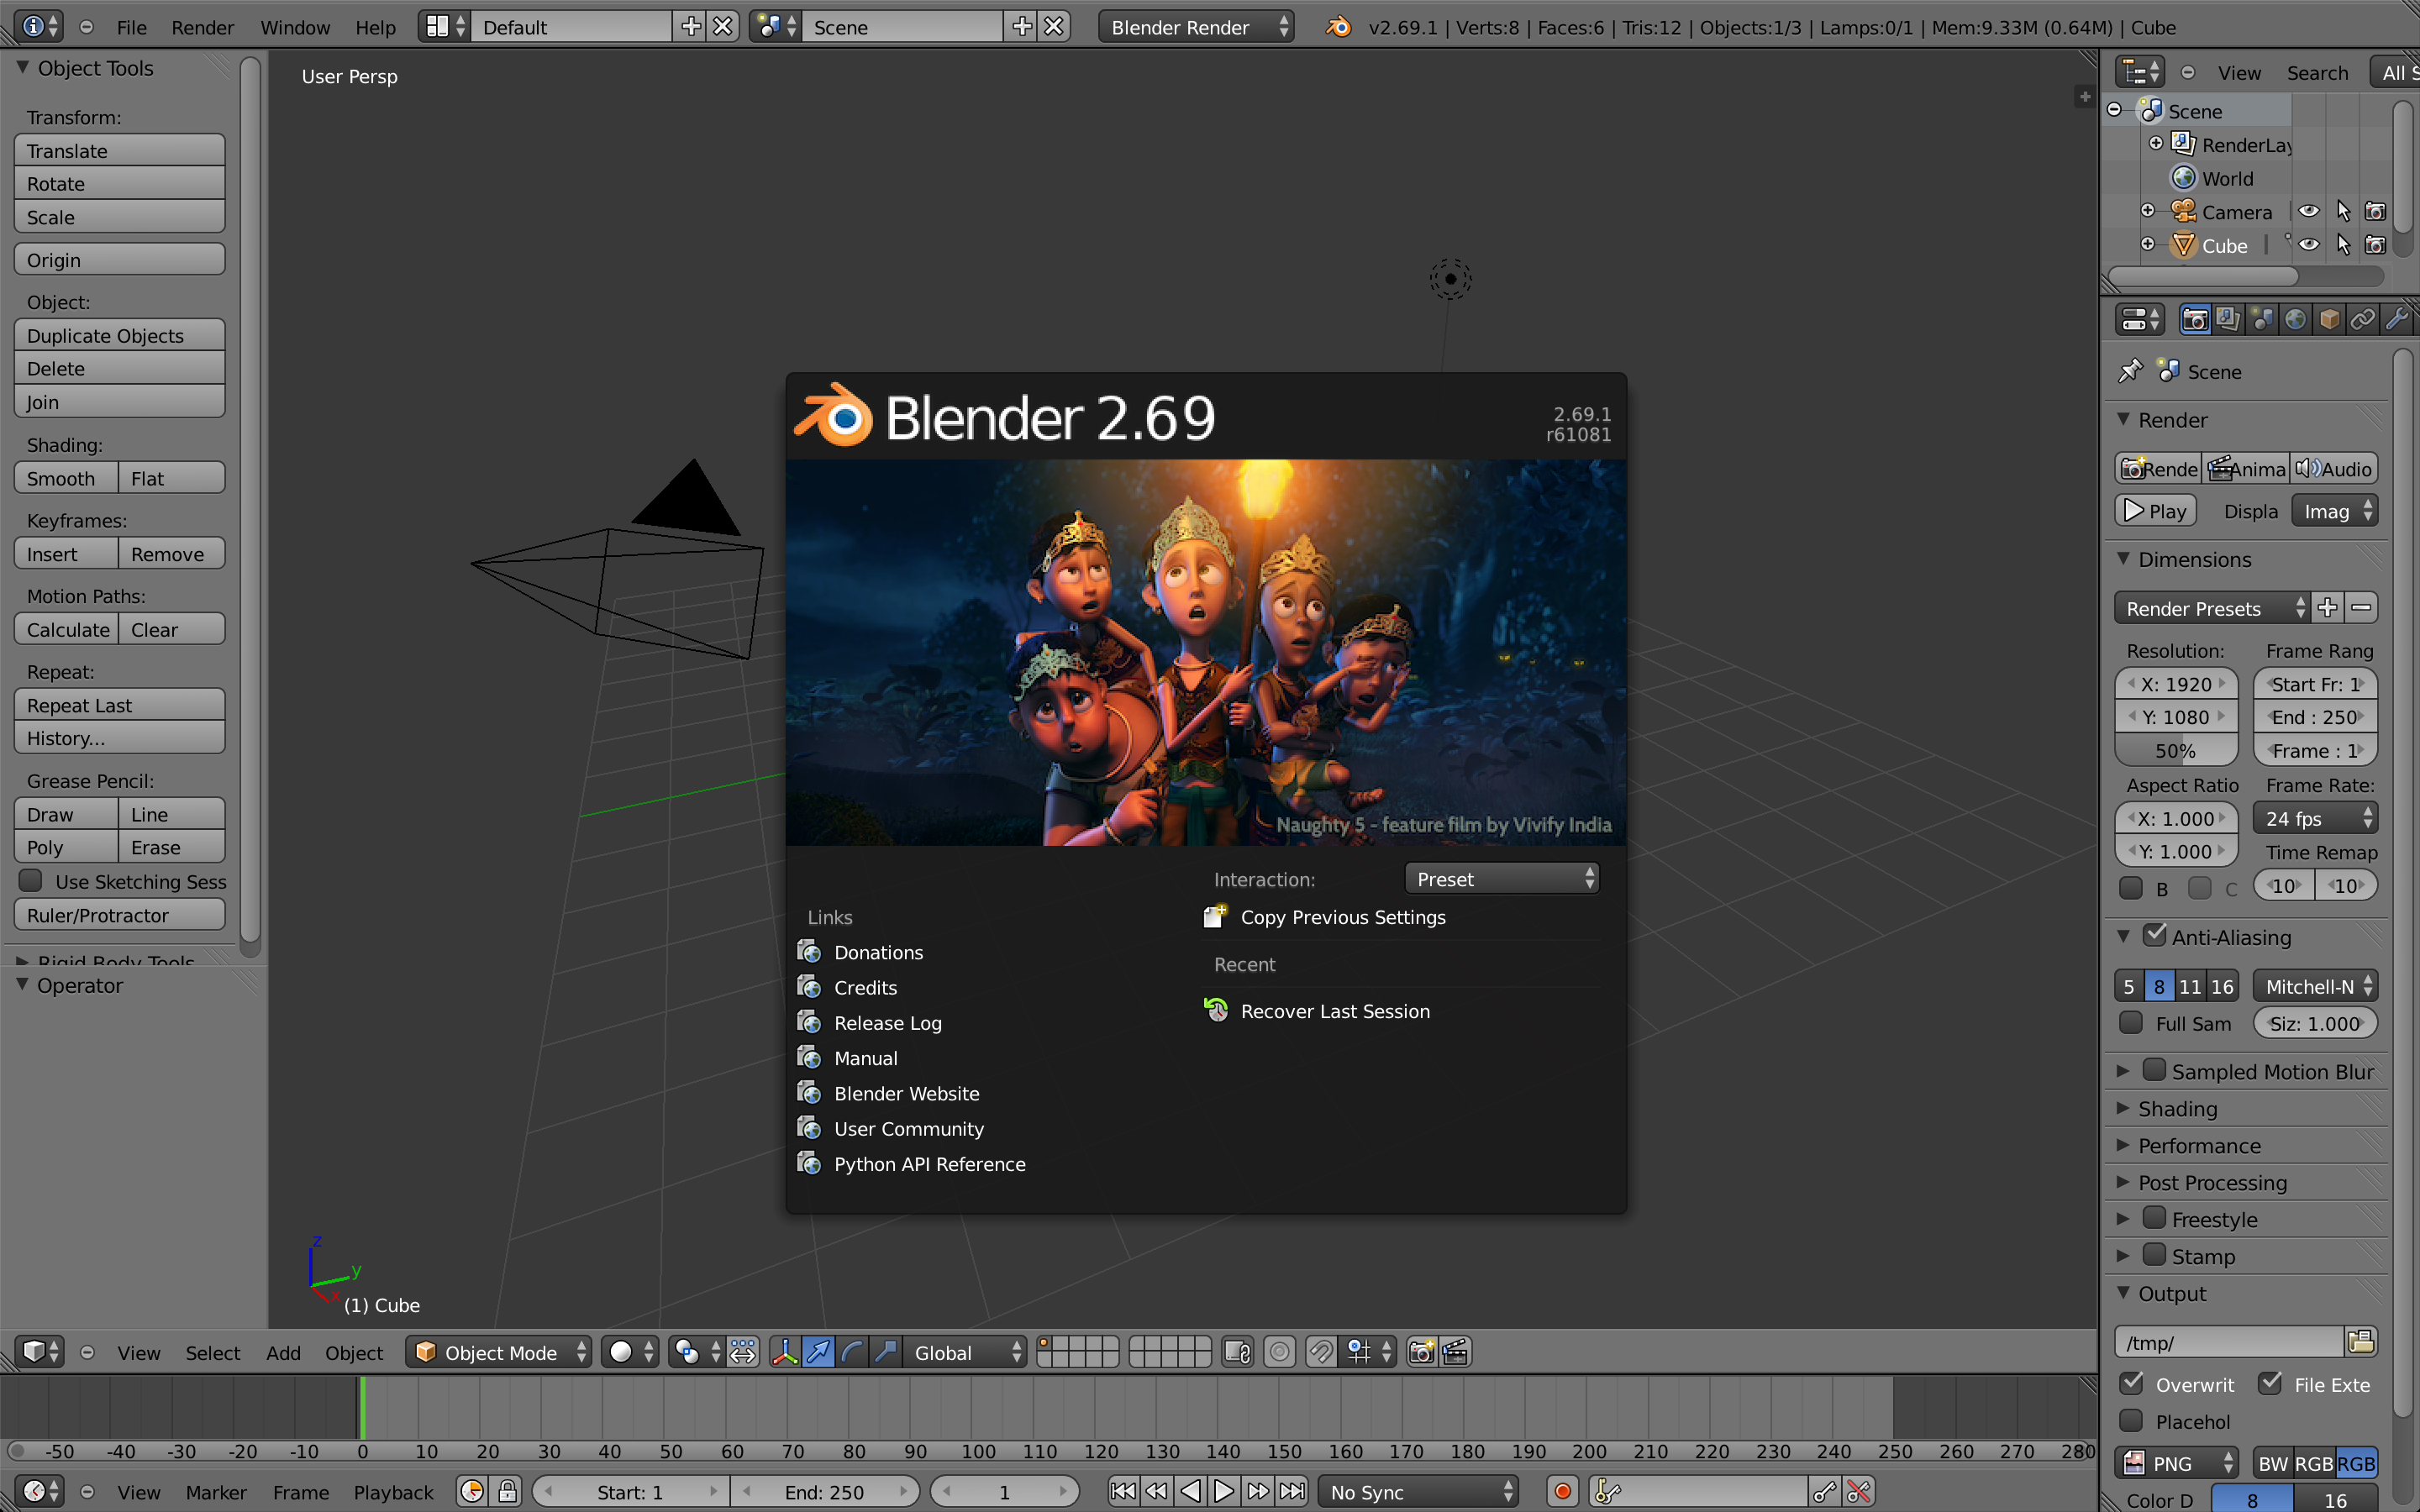
\includegraphics[width=17cm]{blender_gui}
\caption{Interface do Blender, ao abrir a aplicação.}
\label{blender_gui}
\end{figure}

Os principais módulos do Blender são implementados em C, sendo que camadas mais altas usam C++, como a interface gráfica (GUI), que usa OpenGL para não depender dos servidores gráficos de cada plataforma. Os projetos criados no Blender são salvos em arquivos {\it *.blend}, que salvam metadados em cabeçalhos, também a fim de permitir a compatibilidade entre arquiteturas diferentes. Exemplos de metadados salvos são tamanhos de ponteiros, versão do software, e disposição de memória\footnote{Exemplos são {\it little endian} e {\it big endian}.}.

Após o cabeçalho do arquivo, blocos de dados são salvos com informações como códigos identificadores dos objetos na cena, tamanho em memória dos objetos e índices das estruturas de dados que compõe a cena. Cada um destes blocos possuem os vetores de dados com os nomes e tipos de cada objeto, como curvas, malhas, luzes, câmeras, entre outras possibilidades.  

\subsection{Renderização no Blender}

Como o Blender é estruturado de maneira bastante modular, a renderização de uma cena criada no \emph{software} pode ser feita por {\it engines} diferentes, a escolha do usuário. Em uma instalação convencional, o Blender oferece duas \emph{engines} diferentes, mas há suporte para renderizadores de terceiros, com diferentes níveis de integração. \\

As duas \emph{engines} fornecidas são a {\it Blender Internal Render}, às vezes chamada apenas de {\it Blender Render} e o {\it Cycles}.
Elas serão discutidas com maiores detalhes a seguir. Na Figura \ref{renderers}, é mostrado onde, na interface do Blender, a opção por uma engine ou outra pode ser feita. Uma terceira engine, a {\it Blender Game Engine}, também é fornecida, mas engloba muito mais que apenas a geração de imagens, e é usada para a criação de games ou de aplicações interativas, gerando um arquivo executável como resultado. \\

%figura aqui!! :-P
\begin{figure}[!htb]
\center
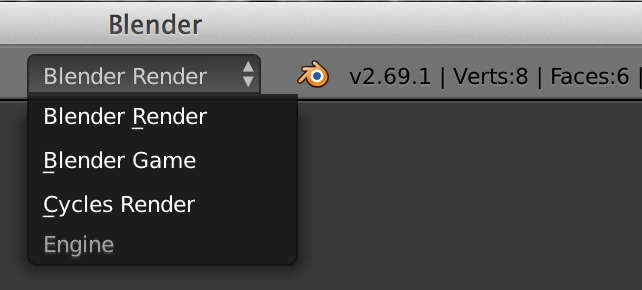
\includegraphics[width=8cm]{blender_render_option}
\caption{Interface do Blender, que permite a escolha de qual engine usar para renderização da cena.}
\label{renderers}
\end{figure}

É possível pré-visualizar a cena, animada ou estática, nas {\it viewports} da aplicação, e estas podem ser em {\it (i)} {\it wireframe}, mostrando apena as arestas dos objetos, {\it (ii)} sólida, preenchendo as superfícies com uma estratégia de {\it shading} simplificada para rápida visualização, ou ainda {\it (iii)} com texturas, permitindo uma visualização mais próxima do resultado final, porém mais lenta de ser obtida e menos interativa, já que o tempo de resposta da interface cai consideravelmente. Quando uma renderização completa e de qualidade final é necessária, todo o modelo de dados do Blender é passado à engine de renderização escolhida, software que, conforme discutido, calcula a emissão, absorção, reflexão e transporte da luz simulada e projeta os resultados sobre um plano de imagem definido pela câmera colocada em cena.

\subsubsection{Blender Internal Render}

A primeira geração de renderizador incluído no Blender, bastante estável, é útil para a geração de imagens em geral, com suporte a renderização volumétrica e a uso da GPU para os cálculos. Esta engine não é fisicamente fiel\footnote{{\bf Fisicamente fiel}, neste contexto, significa que os fundamentos usados para a geração de imagens são as leis da física e suas expressões matemáticas. Unidades e conceitos físicos são usados nos algoritmos e as imagens computadas são ditas fisicamente corretas, isto é, elas correspondem ao comportamento da luz que seria encontrado numa cena real.}, isto é, as unidades e grandezas usadas nas configurações podem usar, e normalmente usam, valores irreais para quantidades de luz. Um exemplo: uma superfície pode refletir 110\% da luz incidente, mesmo quando não é uma superfície emissora de luz.

\subsubsection{Cycles Render}

É uma engine mais moderna, fisicamente fiel, que modela efeitos cáusticos de maneira realista. Tem suporte a configuração de comportamento através de nós e permite que o usuário crie seus próprios shaders em OSL, linguagem apresentada em \ref{osl}. Um exemplo de uma rede de nós para configurar seu comportamento é mostrado na Figura \ref{nodes}. \\

%figura aqui!! :-P
\begin{figure}[!htb]
\center
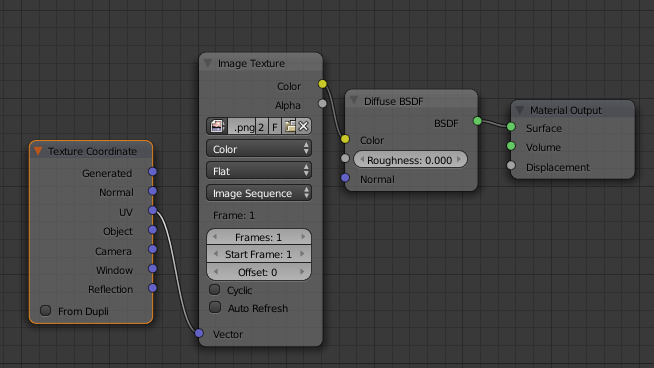
\includegraphics[width=15cm]{Cycles_nodes}
\caption{Rede de nós configurando o uso de uma sequência de imagens como textura para uma superfície.}
\label{nodes}
\end{figure}

Como o software é recente, ele é menos estável e nem todas as funcionalidades desejadas estão disponíveis. Uma das funcionalidades pendentes de implementação é a renderização de volumes, ou volumétrica, assunto deste trabalho.

\section{Texturas}
\label{tex_def}

No processo de modelagem tridimensional, a medida que detalhes se tornam mais sofisticados e complexos, a modelagem explícita de todas as informações desejadas, seja pelo uso de polígonos ou de outras primitivas geométricas, se torna pouco prático e de difícil execução. Uma alternativa é mapear uma imagem à superfície, técnica denominada {\it Mapeamento de Textura}. A imagem utilizada é chamada de {\it textura} e os elementos individuais que compõem a textura são chamados de {\it texels} (\emph{texture elements}, a exemplo do que ocorre com \emph{pixels}). Na imagem resultante, é usual que um \emph{pixel} contenha vários \emph{texels}.

\subsection{Definição}

Textura é um termo bastante amplo em síntese de imagens. De modo geral, podemos dizer que sempre que um ponto é avaliado usando apenas informações locais àquele ponto, trata-se de uma textura. Estas informações locais podem ser a localização do ponto no espaço, sua posição numa superfície, a direção e módulo das derivadas parciais da superfície naquele ponto, entre outras possibilidades. A função avaliada no ponto normalmente retorna um escalar, mas este resultado poderia, a princípio, ser de qualquer tipo, incluindo um vetor ou uma cor. É bastante usual que texturas sejam usadas como parâmetros de funções de {\it shading}.

Uma {\it textura volumétrica} pode ser avaliada em qualquer ponto do espaço; uma {\it textura de superfície} pode ser avaliada apenas sobre os pontos pertencentes à superfície. Além disso, texturas podem ser geradas por um programa e avaliadas sob demanda, ou armazenadas em um arquivo e consultadas para encontrar o valor da textura.

O {\it Mapeamento de Textura}, discutido na próxima seção, descreve a aplicação de uma textura a uma superfície, e determina a relação entre a geometria e o processo de {\it shading}.

\subsection{Mapeamento de Textura}

As texturas são introduzidas nas imagens com o uso de {\it mapeamentos de textura}. É uma forma de adicionar detalhes às superfícies sem que exista um modelo geométrico destes detalhes, de modo a permitir a criação de imagens complexas sem causar um aumento de complexidade na geometria.

De modo geral, mapas de texturas podem ser funções de uma ou mais variáveis. A fim de exemplificar seu funcionamento, mostraremos o caso das funções de duas variáveis.

Um \emph{mapa de textura} associa um {\it texel} a cada ponto no objeto geométrico. Se o objeto for representado por coordenadas homôgeneas, as funções serão dadas por:
\[
	\begin{array}{l}
	x = x(s, t), \\
	y = y(s, t), \\
	z = z(s, t), \\
	w = w(s, t).
	\end{array}
\]

Embora estas funções existam conceitualmente, encontrá-las pode ser difícil. Além disso, o problema mais usual é o inverso: dado o ponto $(x,y,z)$ ou $(x, y, z, w)$ no objeto, desejamos encontrar as coordenadas de textura correspondentes, isto é, as funções inversas 
\[
\begin{array}{l}
s = s(x, y, z, w), \\
t = t(x, y, z, w).
\end{array}
\]

Em computação gráfica, a maioria das superfícies são representadas parametricamente. Um ponto ${\bf p}$ na superfície é uma função de dois parâmetros $u$ e $v$. Para cada par de valores, geramos o ponto

\[
{\bf p}(u,v) = \left[ \begin{array}{c} x(u,v) \\ y(u,v) \\ z(u,v) \end{array} \right].
\]    

Dada uma superfície paramétrica, podemos mapear um ponto do mapa de textura $T(s,t)$ para um ponto ${\bf P}(u,v)$ na superfície usando um mapa linear da forma
\[ \begin{array}{l}
 u = as + bt + c, \\
 v = ds + et + f.
 \end{array}
\]

Neste conjunto de equações, $a$, $b$, $c$, $d$, $e$ e $f$ são coeficientes que definem o mapeamento linear. E se tivermos que $ae \neq bd$, este mapeamento é invertível. 

%figura aqui!! :-P
\begin{figure}[!htb]
\center
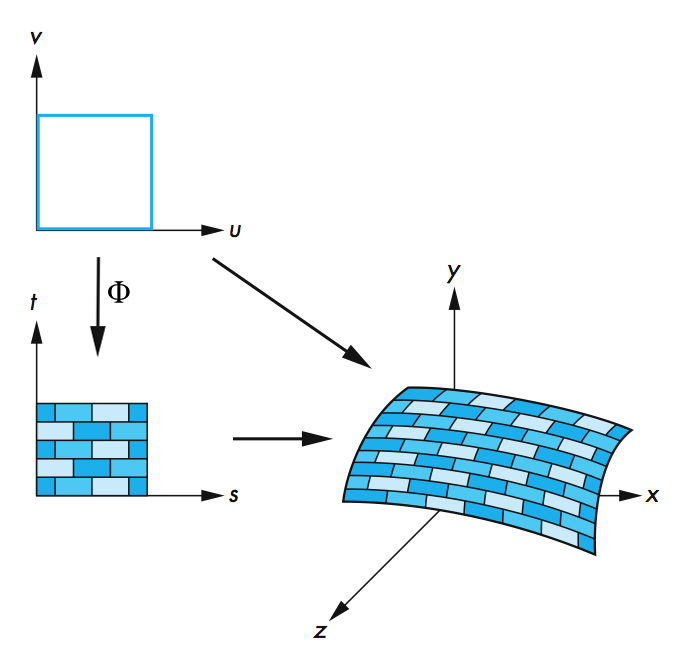
\includegraphics[width=11cm]{tex_mapping}
\caption{Mapeamento do sistema de coordenadas da região parametrizada para o sistema de coordenadas da textura.}
\label{tex_map}
\end{figure}

\subsubsection{Coordenadas de Textura}

Depois de a textura ter sido carregada na memória, ela pode ser amostrada, a fim de se obter uma cor a partir dela. Isso é feito usando \emph{coordenadas de textura}. Usualmente são atributos dos vértices, como posição e cor, armazenados como vetores, que determinam a distância em cada eixo da textura em que a amostra deve ser tomada. o tamanho do vetor depende do número de dimensões que a textura tem - uma textura 2D usa um vetor de pares ordenados para as coordenadas, por exemplo. Estas coordenadas são normalizadas, isto é, independente do tamanho da textura em uso, suas coordenadas variam entre $[0.0, 1.0]$. Como resultado, a aplicação não precisa se preocupar com o tamanho da textura depois que ela foi lida. 

\subsection{Estratégias de \emph{Wrapping}}
Embora texturas sejam definidas como tendo coordenadas normalizadas, os vértices podem usar coordenadas fora deste intervalo. O que ocorre neste caso depende do modo escolhido para {\it wrapping} da textura, que basicamente se refere a como a textura vai ``embrulhar'' a geometria. Um dos modos é denominado \emph{clamping}, que limita os {\it texels} ao tamanho da textura, isto é, se a coordenada solicitada é maior que a textura, a consulta vai retornar o valor da fronteira mais próxima da textura, efetivamente limitando o intervalo válido de consulta ao intervalo $[0.0, 1.0]$. No entanto, se a repetição da textura for permitida, as coordenadas para consulta à textura fazem um \emph{loop} na textura: solicitar o valor da textura no ponto $1.5$, $2.5$ ou até mesmo $100.5$, retorna o valor referente ao meio da textura, de coordenada $0.5$ no eixo considerado. \\

Na API adotada para este trabalho, a estrutura \texttt{Wrap} define os métodos suportados, como mostrado no Código \ref{wrap_enum}. O modo \emph{Black} retorna a cor preta pra qualquer ponto que caia fora do intervalo normalizado, isto é, todo ponto que estiver fora da área da textura, recebe a cor preta como resultado. O modo \emph{Clamp} limita todas as consultas para o intervalo da textura, e retorna o valor da extremidade mais próxima quando o ponto solicitado estiver além da fronteira da textura. Os modos \emph{Periodic} e \emph{Mirror} repetem a textura, sendo que o primeiro repete a textura em sua orientação normal e o segundo reflete a textura em relação a um dos eixos antes de repeti-la.

\begin{figure}[!htb]
\lstinputlisting[label=wrap_enum,caption={Modos de {\it wrapping} suportados pela API.}]{sourceCode/wrap_enum.cpp}
\end{figure}

\subsection{Texturas Tridimensionais}
\label{texturas3d}

A renderização volumétrica (chamaremos de renderização volumétrica o processo de geração de imagens que use uma textura tridimensional) parte da existência de um campo escalar contínuo tridimensional, que pode ser escrito como um mapeamento
\[ \Phi : \mathbb{R}^{3} \rightarrow \mathbb{R},
\]
que é uma função do espaço 3D para um valor de apenas um componente.
Na prática, um campo volumétrico é dado por uma imagem tridimensional, pois trata-se do resultado de uma simulação ou de uma medição. A Figura \ref{grid_ex} mostra um \emph{grid} bidimensional e outro tridimensional, exemplificando os dados para os campos escalares discretos e uniformemente amostrados.

%figura aqui!! :-P
\begin{figure}[!htb]
\center
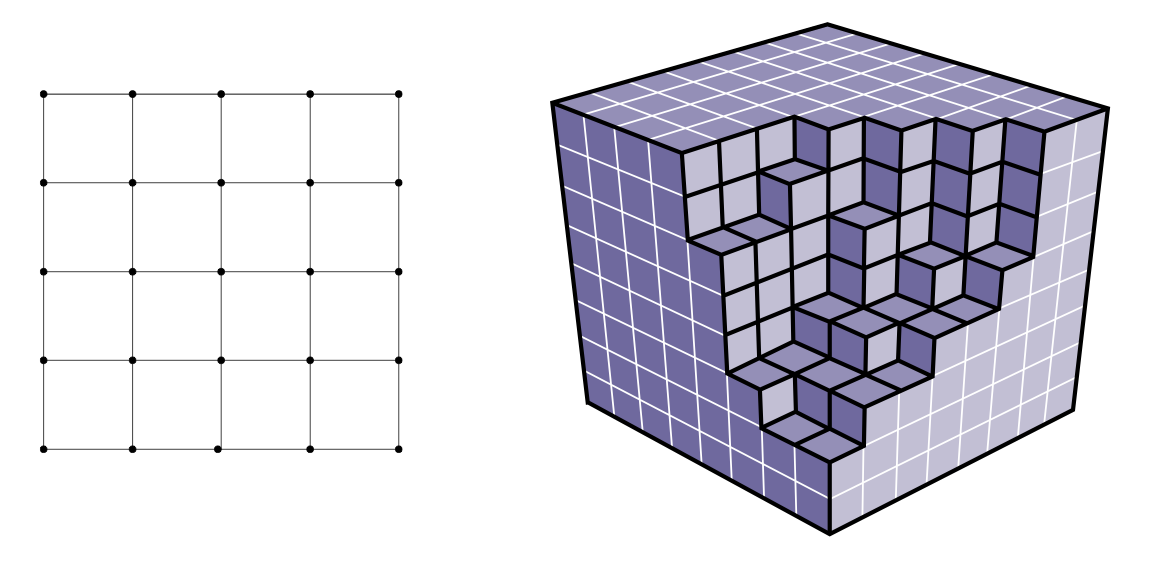
\includegraphics[width=11cm]{grid_example}
\caption{Exemplos de \emph{grids} uniformes: bidimensional com células de razão de aspecto 1, à esquerda, e tridimensional com células cubóides, à direita.}
\label{grid_ex}
\end{figure}

Uma imagem digital bidimensional é um bom exemplo para discutirmos a representação de um volume. Uma imagem consiste de {\it pixels} (abreviação de {\it picture elements}, elementos da figura, em inglês) organizados em um vetor convencional. {\it Pixels} são os elementos de dados de uma imagem 2D, e que possuem valores de cor.
Um conjunto volumétrico discreto pode ser representado de uma maneira similar se levarmos o espaço de duas para três dimensões. Assim, um \emph{pixel} 2D passa a ser um {\it voxel} 3D ({\it volume element}, elemento de volume, em inglês). {\it Voxels} são organizados em um vetor tridimensional convencional também, abrangendo o conjunto de dados que compõe o volume.
Embora seja intuitivo, o termo {\it voxel} tem duas possíveis interpretações. A primeira delas é a de que o {\it voxel} é um pequeno cubo que preenche uma pequena região volumétrica com o valor a ser armazenado. A outra interpretação assume que os {\it voxels} são pontos no espaço de três dimensões, ou seja, sem dimensão, sendo necessário o uso de técnicas de interpolação para preencher os espaços intermediários entre os pontos. Neste trabalho, esta última interpretação se adequa melhor, dada a biblioteca que usamos para representar volumes e as estratégias implementadas para reconstruir os valores nas lacunas entre os pontos definidos. \\

Um \emph{grid} uniforme $n$-dimensional tem a vantagem de ser bem estruturado, o que leva a uma representação compacta na memória do computador (na forma de um vetor $n$-dimensional) e acesso rápido, constante $O(1)$, às celulas. Porém, conforme será discutido no Capítulo \ref{data_struct}, essa representação só é eficiente para os casos em que o volume é denso, isto é, não há predominância de células intermediárias vazias. Além disso, \emph{grids} uniformes não são muito flexíveis, e outras estruturas de volumes podem ser usadas em seu lugar, sendo que apresentaremos uma das possibilidades. \\

\subsubsection{Voxels}

Conforme discutido na seção anterior, podemos acessar o conteúdo de um \emph{voxel} usando suas coordenadas no espaço, da mesma forma que podemos acessar o conteúdo de uma imagem bidimensional. É usual chamarmos as variáveis que representam os índices de $i$, $j$ e $k$ para os eixos $x$, $y$ e $z$, respectivamente. Em notação matemática, é comum a opção por índices subscritos, por exemplo: para um buffer de \emph{voxels}  $B$, dizemos que ele possui \emph{voxesl}  nos pontos amostrais dados por $B_{i,j,k}$. Na implementação, os dados amostrados são acessados usando coordenadas com sinal. Um exemplo é mostrado no Código \ref{vdb_coords}.

\begin{figure}[!htb]
\lstinputlisting[label=vdb_coords,caption={Consulta ao valor de ponto flutuante no voxel de coordenadas (1, 2, 3)}]{sourceCode/vdb_coordinates.cpp}
\end{figure}

\subsubsection{Fonte dos dados de uma textura volumétrica}

Os dados usados para a renderização volumétrica podem ser provenientes de diferentes áreas de aplicação. Um tipo importante de aplicação é a visualização científica de dados escalares. Mais especificamente, a visualização de imagens médicas é uma das aplicações mais proeminentes em visualização. Para obter os dados tridimensionais, usa-se equipamentos de escaneamento não invasivos, como  tomografia computadorizada ou ressonância magnética. \\

Outra fonte corriqueira de dados volumétricos são as simulações numéricas, como as simulações de dinâmica de fluidos, campos magnéticos e de fogo e explosões para efeitos especiais. Neste caso, o \emph{grid} usado para a simulação é normalmente bem diferente daquele usado para visualização. O \emph{grid} usado na simulação pode ser estruturado para garantir uma simulação estável, com características específicas ao fenômeno modelado. \\

Aplicações de visualização normalmente dependem de um \emph{grid} uniforme, que facilita métodos rápidos de geração de imagens. Desta forma, é usual que grids resultantes de simulações sejam transformados antes de fornecidos a um renderizador volumétrico. 

\subsubsection{Reconstrução}

Como um conjunto volumétrico de dados é representado de forma discreta, existe o problema de reconstruirmos uma função escalar em todos os pontos do domínio 3D.
O problema de uma reconstrução fiel é estudado em processamento de sinais. \\

Pelo teorema de amostragem de Nyquist-Shannon da teoria da informação, temos que a frequência do sinal de entrada precisa ser maior que o dobro da frequência máxima que ocorre no sinal de entrada para que o sinal original possa ser reconstruído a partir do sinal amostrado. Caso contrário, o sinal apresentará problemas de serrilhamento (\emph{aliasing}), isto é, o sinal contínuo será reconstruído com erros a partir do sinal discreto. \\

Em notação matemática, a amostragem apropriada pode ser descrita da seguinte forma: para um sinal de entrada periódico e contínuo representado pela função $f(t)$, determinamos primeiro sua frequência máxima $v_{f}$. Frequência máxima significa que a transformada de Fourier de $f(t)$ é zero fora do intervalo de frequências $[-v_{f}, v_{f}]$. Com isso, temos a frequência crítica de amostragem (também chamada de frequência Nyquist) $v_{N} = 2v_{f}$. Para uma amostragem apropriada, mais que $2v_{f}$ amostras precisam ser tomadas por unidade de distância. Para uma amostragem uniforme numa frequência $v_{s}$, os pontos amostrais podem ser descritos por $f_{i} = f(i/v_{s})$, com $i$ inteiros. \\

Dado que o sinal original é amostrado numa frequência $v_{s} > v_{N}$, o sinal pode ser recuperado das amostras $f_{i}$ conforme abaixo:
\[
	f(t) = \sum_{i} f_{i}\;sinc(\pi (v_{s}t - i)).
\]

A função $sinc(x)$ (de {\it sinus cardinalis}, seno cardinal, em latim) é dada por:
\[
	sinc(t) = \left\{ 
	\begin{array}{cl} 
	\frac{sen(t)}{t} & se\;\; t \neq 0  \\
	1 & se\;\; t = 0
	\end{array} \right. 
\]

Um sinal cuja transformada de Fourier é zero fora do intervalo de frequências $[-v_{f}, v_{f}]$ é chamado de limitado em banda porque sua largura de banda (isto é, sua frequência) é limitada. Na prática, as frequências que ocorrem num dado conjunto de dados podem ser desconhecidas. Nestes casos, um filtro passa-baixa pode ser aplicado para restringir a frequência máxima em um valor controlado. \\

A $f(t)$ apresentada é um exemplo de convolução, e descreve a convolução do sinal amostrado de entrada $f_{i}$ com um filtro $sinc$. Na realidade, porém, o filtro $sinc$ possui alcance ilimitado, isto é, ele oscila em torno de zero sobre todo o domínio. Como consequência, a convolução precisa ser calculada para todas as amostras de entrada $f_{i}$, o que toma muito tempo. É por isso que na prática aplica-se filtros de reconstrução com suporte finito.

Um exemplo é o filtro {\it caixa}, que leva à interpolação do vizinho mais próximo quando a largura da caixa é igual à distância de amostragem (isto é, o valor da função reconstruída é dado pelo valor do ponto amostral mais próximo). Outro exemplo é o filtro {\it triangular}, que leva a uma reconstrução linear quando a largura de um lado for igual à distância de amostragem. A Figura \ref{filters} mostra três tipos diferentes de filtros de reconstrução que podem ser usados. \\

%figura aqui!! :-P
\begin{figure}[!htb]
\center
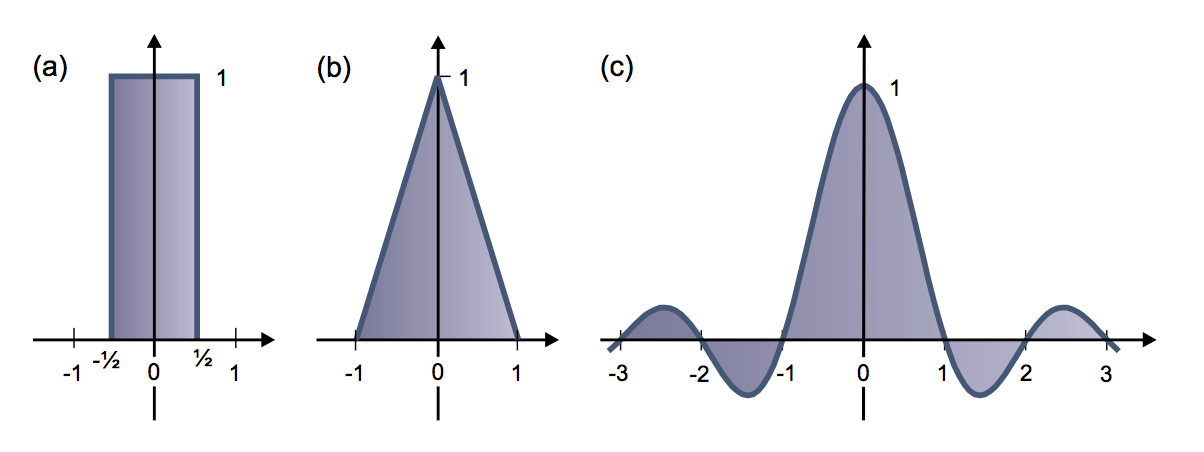
\includegraphics[width=15cm]{recon_filters}
\caption{Exemplos de filtros de reconstrução: (a) filtro caixa, (b) filtro triangular, e (c) filtros que usam o seno cardinal, {\it sinc}.}
\label{filters}
\end{figure}

Embora tenhamos discutido funções de apenas uma variável, podemos extender a discussão para $n$ dimensões usando uma abordagem de produto tensorial. A idéia é basicamente fazer a reconstrução de cada dimensão, mas de forma combinada. Para o nosso caso, em que precisamos de três dimensões, um filtro de reconstrução usando produto tensorial é dado por $h(x,y,z) = h_{x}(x)\;h_{y}(y)\;h_{z}(z)$, onde $h_{x}(\cdotp)$, $h_{y}(\cdotp)$ e $h_{z}(\cdotp)$ são filtros de um único parâmetro ao longo dos eixos $x$, $y$ e $z$. E uma das vantagens do uso de um \emph{grid} uniforme é que eles dão suporte a este tipo de reconstrução de forma direta. Como mostrado na Figura \ref{produtoTensorial}, a abordagem de produto tensorial separa as interpolações ao longo de cada dimensão e permite o cálculo do valor reconstruído através de uma sequência de interpolações lineares.

%figura aqui!! :-P
\begin{figure}[!htb]
\center
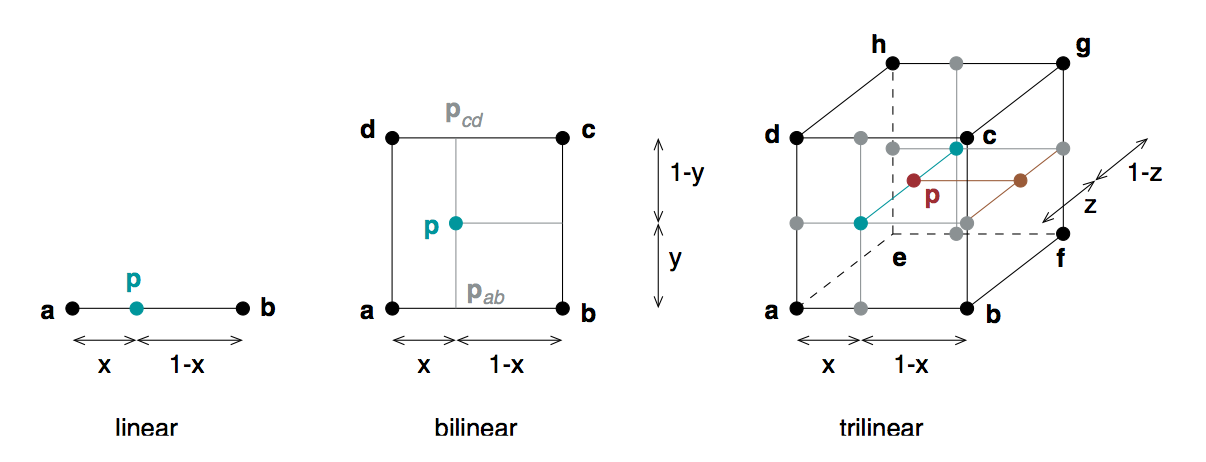
\includegraphics[width=15cm]{produtoTensorial}
\caption{Interpolações lineares usando o produto tensorial: casos linear, bilinear e trilinear.}
\label{produtoTensorial}
\end{figure}

\subsubsection{Filtros e Técnicas de Interpolação}

Quando desejamos aplicar uma textura 2D à superfície de uma geometria 3D, por exemplo, é bastante improvável que haja uma correspondência exata de $1:1$ entre os {\it texels} da textura e os {\it pixels} da tela ou da imagem a ser gerada. Duas possibilidades existem neste caso: quando uma textura é amostrada, o {\it texel} mais próximo do ponto solicitado pode ser retornado, ou uma \emph{interpolação} pode ser aplicada a um grupo de {\it texels} para que um valor possa ser calculado e retornado. \\

O exemplo mais simples de um filtro de textura no caso bidimensional é a \emph{Interpolação Bilinear} - os {\it texels} mais próximos nos eixos $x$ e $y$ são considerados a fim de calcular a cor final. \\

Para o caso de texturas tridimensionais, desejamos consultar o valor de um {\it voxel}. Pelo uso de coordenadas $(i, j, k)$ podemos acessar {\it voxels} individuais, mas a princípio, isso funciona apenas quando o ponto que desejamos amostrar corresponde exatamente ao centro do {\it voxel}. Em todos os outros casos, uma estimativa precisa ser feita acerca do valor, a ser definido pelos {\it voxels} vizinhos ao ponto que buscamos. As principais técnicas de interpolação serão discutidas a seguir. \\

\emph{Interpolação do vizinho mais próximo}. Em inglês, interpolação \emph{Nearest-Neighbor}. Trata-se da forma mais simples de interpolação, e pode-se dizer até que, de tão simples, não se qualifica como uma técnica de interpolação. Ao invés de considerar valores de {\it voxels} vizinhos, este método considera apenas o valor do centro do {\it voxel} que estiver mais próximo do ponto solicitado. Como consequência, a imagem resultante mostra claramente as fronteiras de cada {\it voxel}. 

Dada uma função discretamente amostrada {\bf d} e uma posição $x$, a interpolação do vizinho mais próximo em uma dimensão pode ser escrita como
\[
I_{n}(x, {\bf d}) = {\bf d}_{\floor*{x+0.5}}.
\]

Em código, temos um vetor unidimensional $A$ e uma coordenada de ponto flutuante $x$. Assumindo que $x$ está dentro do intervalo válido de $A$, a implementação é mostrada no Código \ref{nearestNeighbor}. O comportamento desta técnica de interpolação é ilustrado pela Figura \ref{nearestNeighborImage}. A implementação para o caso tridimensional é mostrado no código \ref{nearestNeighbor3d}. \\

\begin{figure}[!htb]
\lstinputlisting[label=nearestNeighbor,caption={Implementação da interpolação do vizinho mais próximo.}]{sourceCode/nearestNeighbor.cpp}
\end{figure}

%figura aqui!! :-P
\begin{figure}[!htb]
\center
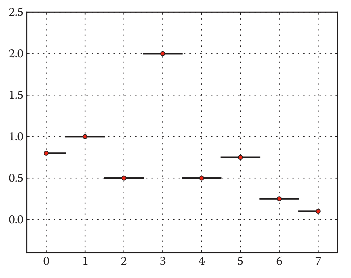
\includegraphics[width=9cm]{nearestNeighbor}
\caption{Interpolação do vizinho mais próximo. Os segmentos de reta mostram todo o intervalo que seria resolvido ao ponto denotado por cada círculo.}
\label{nearestNeighborImage}
\end{figure}


\begin{figure}[!htb]
\lstinputlisting[label=nearestNeighbor3d,caption={Implementação da interpolação do vizinho mais próximo para o caso tridimensional.}]{sourceCode/nearestNeighbor3d.cpp}
\end{figure}

\emph{Interpolação Linear}. Entre as técnicas de interpolação que usam valores intermediários para o cálculo, a interpolação linear é o caso mais simples. Os valores são calculados considerando os pontos próximos do ponto consultado e usando ponderação em função da distância, de modo que a contribuição de um ponto amostral é igual a $1.0$ se o ponto consultado está alinhado com o centro do voxel e é $0.0$ quando a distância do ponto consultado até o centro do voxel é $1.0$.

Dada a mesma função {\bf d} e coordenada $x$ do caso anterior, a interpolação linear pode ser escrita da seguinte forma:
\begin{center}
\[I_{l}(x, {\bf d}) = (1 - \alpha) \cdotp {\bf d}_{\left\lfloor x \right\rfloor} + \alpha \cdotp {\bf d}_{\left\lceil x \right\rceil}, \]
\[
\alpha = x - \left\lfloor x \right\rfloor.\]
\end{center}

A implementação é apresentada para o caso unidimensional no Código \ref{linear1d}. Para o caso tridimensional, há mais a ser feito. Os índices discretos precisam ser encontrados da mesma forma que no caso da interpolação pelo vizinho mais próximo, mas ao contrário daquele caso, precisamos agora dos valores de oito \emph{voxels} vizinhos, ao invés de apenas um. De modo geral, quanto maior a vizinhança que precisa ser considerada na interpolação, mais lento o processo. Definimos como \emph{Suporte} (denotado por $S$) o número de vizinhos a serem considerados numa dada técnica de interpolação. Para interpolação linear, temos $S = 2$. O número de valores de \emph{voxel} que uma técnica de interpolação precisa é dado por $2^{n}$, em que $n$ é o número de dimensões. Logo, para nosso caso, interpolação linear em três dimensões, o número de amostras necessário é $2^{3} = 8$. Na Figura \ref{linearInterp}, pode parecer que as descontinuidades indicam as fronteiras dos \emph{voxels} considerados, mas na realidade, a descontinuidade ocorre quando o ponto sendo amostrado passa de um intervalo $[r_{i-1}, r_{i}]$ para um intervalo $[r_{i}, r_{i+1}]$, e isso ocorre nos centros dos \emph{voxels}, e não nas fronteiras.

\begin{figure}[!htb]
\lstinputlisting[label=linear1d,caption={Implementação da interpolação linear para uma dimensão.}]{sourceCode/linear1d.cpp}
\end{figure}

%figura aqui!! :-P
\begin{figure}[!htb]
\center
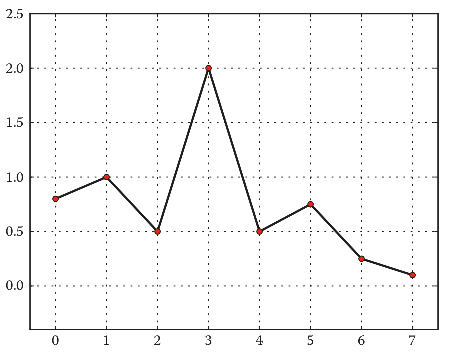
\includegraphics[width=9cm]{linear}
\caption{Interpolação linear. As quebras ocorrem na transição do centro de um voxel para o centro do voxel seguinte.}
\label{linearInterp}
\end{figure}

A implementação do caso tridimensional é apresentada no Código \ref{linear3d}. \\

%\begin{minipage}{\textwidth}
\begin{figure}[!htb]
\lstinputlisting[label=linear3d,caption={Implementação da interpolação linear para três dimensões.}]{sourceCode/linear3d.cpp}
\end{figure}
%\end{minipage}

\emph{Interpolação Cúbica}. A última técnica de interpolação que trataremos é a interpolação cúbica. A interpolação linear usa um polinômio de primeira ordem (linear) para calcular os valores intermediários, mas seu resultado, embora não seja ruim como a interpolação do vizinho mais próximo, ainda é pouco suave. Se usarmos polinômios de ordens maiores, obteremos resultados melhores, isto é, com transições mais suaves, ao custo de velocidade, já que o tempo de cálculo aumentará. 

O próximo passo, depois da interpolação linear, é a interpolação cúbica, que usa quatro valores vizinhos para a interpolação:
\[
 I_{c} (x, P_{i-1}, P_{i}, P_{i+1}, P_{i+2}).
\]  

Para derivar a fórmula da interpolação cúbica, consideramos a forma básica de um polinômio de terceira ordem e sua derivada:
\[
\begin{array}{l}
	f(x) = ax^3 + bx^2 + cx + d \\
f'(x) = 3ax^2 + 2bx + c.
\end{array}
\]
Os pontos que desejamos interpolar estão no intervalo $[0, 1]$, e os quatro pontos que funcionam como entrada para a função de interpolação são
\[
\begin{array}{rcl}
P_{i-1} & = & -1, \\
P_{i} & = & 0, \\
P_{i+1} & = & 1, \\
P_{i+2} & = & 2.
\end{array} 
\]

Calculando a função e sua derivada em $0$ e $1$, obtemos

\[
\begin{array}{rcl}
f(0) & = & d, \\
f(1) & = & a + b + c + d, \\
f'(0) & = & c, \\
f'(1) & = & 3a + 2b + c.
\end{array} 
\]

Reescrevendo cada um dos resultados de modo a isolar $a$, $b$, $c$ e $d$, obtemos
\[
\begin{array}{rcl}
a & = & 2f(0) - 2f(1) + f'(0) + f'(1), \\
b & = & -3f(0) + 3f(1) - 2f'(0) - f'(1), \\
c & = & f'(0), \\
d & = & f(0).
\end{array} 
\]

Sabemos os valores de $f(0)$ e de $f(1)$, mas os valores das derivadas não são dados diretamente à função. Porém, como temos $f(-1)$ e $f(2)$, podemos calculá-las:
\[
\begin{array}{rcl}
f(0) & = & P_{i}, \\
f(1) & = & P_{i+1}, \\
f'(0) & = & \frac{P_{i+1} - P_{i-1}}{2}, \\
f'(1) & = & \frac{P_{i+2} - P_{i}}{2}.
\end{array} 
\]

Combinando os dois últimos conjuntos de equações, encontramos os valores de $a$, $b$, $c$ e $d$ em sua forma simples e fechada:
\[
\begin{array}{rcl}
a & = & -\frac{1}{2}P_{i-1} +\frac{3}{2}P_{i} +\frac{3}{2}P_{i+1} +\frac{1}{2}P_{i+2}, \\
b & = & P_{i-1} +\frac{5}{2}P_{i} + 2P_{i+1} -\frac{1}{2}P_{i+2}, \\
c & = & -\frac{1}{2}P_{i-1} + \frac{1}{2}P_{i+1}, \\
d & = & P_{i},
\end{array} 
\]

o que nos leva à solução do problema original,


\begin{align*}
 I_{c} (x, P_{i-1}, P_{i}, P_{i+1}, P_{i+2}) = \left( -\frac{1}{2}P_{i-1} +\frac{3}{2}P_{i} +\frac{3}{2}P_{i+1} +\frac{1}{2}P_{i+2} \right)x^3 &+ \\
 \left( P_{i-1} +\frac{5}{2}P_{i} + 2P_{i+1} -\frac{1}{2}P_{i+2} \right)x^2 &+ \\ \left( -\frac{1}{2}P_{i-1} + \frac{1}{2}P_{i+1} \right)x &+ \\ P_{i}.
 \end{align*}

A interpolação cúbica usa dois valores abaixo e dois acima do ponto consultado, então a técnica tem um suporte $S = 4$, como é possível visualizar na Figura \ref{cubicInterp}. Em três dimensões, o custo total é dado por $4^3 = 64$ consultas para o cálculo de um único valor. No Código \ref{cubic}, a implementação é dada para uma, duas e três dimensões. A implementação de uma dimensão maior sempre usa a função definida para uma dimensão menor.

Uma das desvantagens da interpolação cúbica é que encontramos casos de {\it overshoots}. Quando temos grandes gradientes nos dados discretos, a técnica pode assumir valores maiores ou menores que qualquer um dos dados existentes em todo o conjunto. Dado o escopo deste trabalho, consideraremos que os problemas que isso acarreta são aceitáveis na geração de imagens para nossa aplicação.

%figura aqui!! :-P
\begin{figure}[!htb]
\center
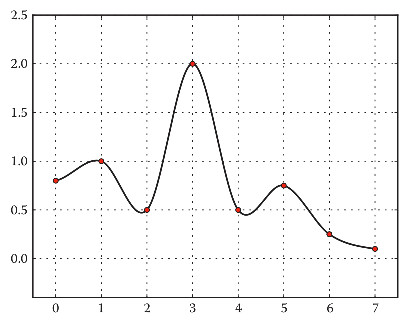
\includegraphics[width=9cm]{cubic}
\caption{Interpolação cúbica. Como o polinômio é de terceira ordem, as curvas são bem mais suaves que da interpolação linear.}
\label{cubicInterp}
\end{figure}

\begin{figure}[!htb]
\lstinputlisting[label=cubic,caption={Implementação da interpolação cúbica para uma, duas e três dimensões.}]{sourceCode/cubic.cpp}
\end{figure}

\section{Sistemas de Coordenadas}

É bastante natural que o conceito de Sistemas de Coordenadas permeie as aplicações de computação gráfica. Afinal, é bastante usual criar um objeto em seu próprio sistema de coordenadas, chamado de sistema de coordenadas de modelagem do objeto, e posteriormente colocar este objeto em uma cena usando as coordenadas do mundo. O objetivo principal de existirem vários sistemas de coordenadas é permitir uma execucação mais eficiente de cada passo do processo de visualização. Para este fim, os objetos precisam ser transformados para sistemas de coordenadas (ou espaços de referência) nos quais as tarefas inerentes a cada etapa do processo seja mais natural e conveniente. O processo gráfico completo, do modelo até a exibição da imagem em um monitor envolve o uso de 7 espaços diferentes. São eles os espaços do objeto, da cena ou do mundo, da câmera, espaço normalizado, de ordenação, de imagem e do dispositivo. Comentaremos apenas acerca dos dois espaços mais relevantes a esse trabalho, mas um tratamento completo pode ser encontrado em \cite{ANGEL}.

\subsubsection{Espaço do objeto}
Também chamado de espaço do modelo, é o sistema de coordenadas em que um objeto 3D específico está definido. Normalmente, embora não sempre, cada objeto terá seu próprio espaço de objeto com origem no centro do objeto em questão. Por centro, entenda-se o ponto em torno do qual o objeto é movido e rotacionado, como um pivô, e que pode não coincidir com o centro geométrico do objeto. Um exemplo é mostrado na Figura \ref{objectSpace}.

%figura aqui!! :-P
\begin{figure}[!htb]
\center
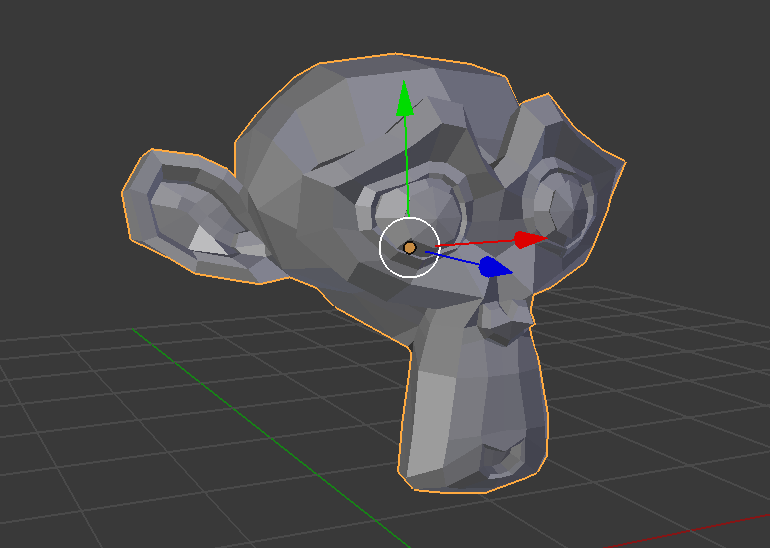
\includegraphics[width=7cm]{objectSpace}
\caption{Espaço do objeto.}
\label{objectSpace}
\end{figure}

\subsubsection{Espaço da cena}
Espaço da cena, também chamado de espaço do mundo, ou ainda de sistema de coordenadas global, é o sistema de coordenadas do universo tridimensional em consideração. Nele, os objetos do cenário são posicionados e orientados, uns em relação aos outros, incluindo a câmera virtual. Um exemplo é mostrado na Figura \ref{worldSpace}.


%figura aqui!! :-P
\begin{figure}[!htb]
\center
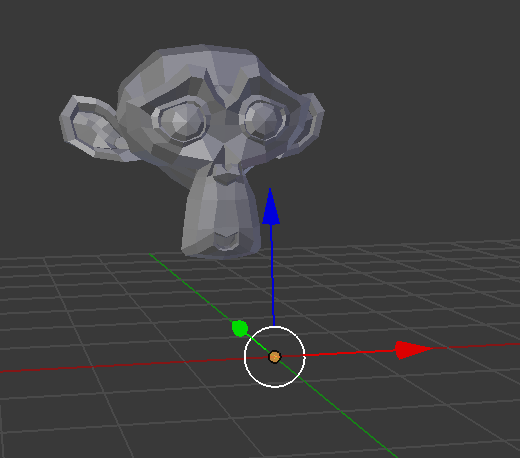
\includegraphics[width=7cm]{worldSpace}
\caption{Espaço da cena, com a origem centrada no círculo menor.}
\label{worldSpace}
\end{figure}

\subsection{Notação Homogênea}

Um ponto descreve um local no espaço, ao passo que um vetor descreve uma direção e não possui localização. Usando matrizes $3 \times 3$ (ou, eventualmente, $2 \times 2$ para duas dimensões), é possível aplicar transformações lineares como rotações, escala e cisalhamento às coordenadas. Contudo, translações não são possíveis com o uso destas matrizes. Essa característica não afeta operações com vetores, mas a translação é uma operação importante para pontos.


A notação homogênea é útil para transformar tanto vetores quanto pontos, e nos permite aplicar translações apenas aos pontos. As matrizes $3 \times 3$ são aumentadas para $4 \times 4$ e pontos tridimensionais e vetores passam a ter um elemento a mais. Assim, um vetor homogêneo é representado por ${\bf p} = (p_{x}, p_{y}, p_{z}, p_{w})$. Nestas condições, $p_{w} = 1$ para pontos e $p_{w} = 0$ para vetores. Quando lidamos com projeções, outros valores podem ser usados para $p_{w}$. Dessa forma, quando $p_{w} \neq 0$ e $p_{w} \neq 1$, precisamos homogeneizar o vetor, e fazemos $(\frac{p_{x}}{p_{w}}, \frac{p_{y}}{p_{w}}, \frac{p_{z}}{p_{w}}, 1)$ a fim de obter o ponto que de fato desejamos. No caso mais simples, $M$ é tal como mostrada abaixo.

\[ M_{4 \times 4} = \left(
\begin{array}{cccc}
m_{00} & m_{01} & m_{02} & 0 \\
m_{10} & m_{11} & m_{12} & 0 \\
m_{20} & m_{21} & m_{22} & 0 \\
0 & 0 & 0 & 1 
\end{array} \right)
\]

As matrizes específicas das transformações de rotação, escala e cisalhamento podem substituir a matriz $M$ apresentada, e estas operações afetarão pontos e vetores, como esperado. Uma translação, contudo, usa os elementos adicionais da matriz aumentada para obter o resultado necessário. Uma matriz de translação, $T$, que translada um ponto por um vetor $t$, é mostrada abaixo.

\[ T = \left(
\begin{array}{cccc}
1 & 0 & 0 & {\it t_{x}} \\
0 & 1 & 0 & {\it t_{y}} \\
0 & 0 & 1 & {\it t_{z}} \\
0 & 0 & 0 & 1 
\end{array} \right)
\]

A combinação de uma transformação linear seguida de uma translação é denominada {\it transformada afim}.

Verificamos com facilidade que um vetor ${\bf v} = (v_{x},v_{y},v_{z},0)$ não é afetado pela transformação ${\bf Tv}$ porque seu último elemento é 0. Se ao ponto $P= (P_{x},P_{y},P_{z},1)$ aplicarmos a transformada ${\bf T}P$, o resultado que obtemos é $P = (P_{x} + t_{x},P_{y} + t_{y},P_{z} + t_{z},1)$, ou seja, o ponto $P$ transladado por $t$.

Como é de se esperar, multiplicações entre matrizes e multiplicações entre matrizes e vetores são calculadas normalmente, sem alterar o que foi discutido.


\section{\emph{Shaders}}
\label{shaders}

Um \emph{shader} é um programa com entradas e saídas, que executa uma tarefa específica no processo de renderização de uma cena, como determinar a aparência de um material ou o comportamento de uma luz. O código fonte do programa é escrito em uma linguagem altamente dependente do ambiente alvo. Exemplos incluem a OpenGL Shading Language (GLSL) e a Direct3D High Level Shader Language (D3D-HLSL). Neste trabalho, a linguagem de \emph{shading} adotada é a Open Shading Language, discutida na Seção \ref{osl}.\\

De modo geral, \emph{shaders} são programas bastante simples que descrevem as características de um vértice ou de um \emph{pixel}. \emph{Shaders} de vértice descrevem as características de um vértice, como posição, coordenadas de textura, cores, entre outras características. \emph{Shaders} de \emph{pixel} descrevem informações como cor, profundidade (\emph{z-depth}, quando um \emph{z-buffer}\footnote{Algoritmo que implementa uma solução adotada para o problema de visibilidade tridimensional quando uma cena é transformada para as coordenadas de tela, e a profundidade relativa entre os objetos precisa ser estabelecida.} está sendo usado), transparência, entre outras possibilidades. 


\subsection{\emph{Open Shading Language}}
\label{osl}

A \emph{Open Shading Language} (OSL) é uma linguagem sucinta, apesar de bastante completa, para a programação de \emph{shaders} em renderizadores modernos e aplicações semelhantes, e é ideal para descrever materiais, luzes, deslocamentos e geração de padrões.
A linguagem foi desenvolvida pela Sony Pictures Imageworks para uso em seu renderizador proprietário para animação de longa-metragens e efeitos visuais. A especificação da linguagem foi desenvolvida com a participação de outras empresas produtoras de animação e efeitos especiais e que também possuíam interesse em utilizá-la.
A licença utilizada é a nova-BSD, de 1999, o que permite seu uso em qualquer aplicação gratuita ou comercial, aberta ou proprietária, bem como modificação do código fonte. \\

A OSL tem uma sintaxe parecida com a do C, e parecida também com outras linguagens de \emph{shading}. No entanto, ela foi escrita especificamente para algoritmos modernos de renderização e suporta \emph{closures}\footnote{Função ou referência a uma outra função, dotada de um ambiente de referência. Isto é, permite que uma função acesse variáveis não locais mesmo quando chamada fora de seu escopo léxico imediato.} para cálculo de cores, BSDFs\footnote{\emph{Bidirectional scattering distribution function}, função de distribuição bidirecional de propagação, em tradução livre. Trata-se da função que descreve como a luz é propagada por uma superfície.} e \emph{ray-tracing} postergado, com avaliação dos raios em momento posterior do processo de geração da imagem. \\

Uma das principais características desta linguagem é que o resultado dos \emph{shaders} de superfície e de volume são \emph{closures}, e não cores resultantes, o que seria mais habitual.
No entanto, temos que os \emph{shaders} escritos em OSL calculam uma descrição simbólica explícita, o \emph{closure}, para descrever como a superfície ou o volume propaga a luz, em unidades radiométricas. Estes \emph{closures} podem ser avaliados em mais de uma direção de propagação de luz, podem ser amostrados para encontrar direções importantes numa dada cena, ou armazenados para avaliação posterior pelo renderizador que está rodando o \emph{shader}. Esta abordagem é ideal para renderizadores que tentam ser fiéis ao comportamento físico da luz, especialmente para os que suportam \emph{ray-tracing}\footnote{Técnica de geração de imagens que se baseia em traçar raios de luz através dos \emph{pixels} no plano da imagem e simular os efeitos de suas interações com os objetos da cena modelada.} e iluminação global\footnote{\emph{Global Illumination} (GI) abrange as técnicas que consideram em adição à iluminação direta a iluminação indireta, como a reflexão da luz em outros objetos.}.


\begin{figure}[!htb]
\lstinputlisting[label=osl_struct,caption=Estrutura de um shader escrito em OSL.]{sourceCode/osl_structure.cpp}
\end{figure}